\citeonline{mclean_visualisation_2010} corrobora com definição de \emph{live coding}  \citeonline{blackwell_programming_2005}. Enquanto primeiro afirma que o \emph{live coding} é uma  ``improvisação de vídeo e/ou música usando \textbf{linguagens de computador} que tem se desenvolvido em um campo ativo de pequisa e prática artística ao longo da última década'' \footnote{Tradução parcial nossa de: \emph{Live coding , the improvisation of video and/or music using computer language, has developed into an active field of research and arts pratice over the last decade}. Grifo nosso}, o segundo descreve como um construto social que derivou em um Programa de Investigação Científica (PIC):

\begin{citacao} 
Nos anos recentes houve uma expansão da atividade do \emph{live coding}, e a formação de um corpo internacional para suportar \emph{live coders} - TOPLAP. O sítio \url{toplap.org} e sua lista de email é a mais ativa casa para práticas artístcas, e o TOPLAP tem sido listado para tais festivais de música eletrônica como Ultrasound (2004), transmediale 2005 (Berlin) e Sonar 2005 (Barcelona) \cite[p.~3-4]{blackwell_programming_2005}.\footnote{Tradução parcial de: \emph{Recent years have seen further expansion of live coding activity, and the formation of an international body to support live coders- TOPLAP (Ward et al. 2004). The toplap.org site and mailing list is the most active current home for this artistic practice, and TOPLAP have been booked for such electronic music festivals as Ultrasound 2004 (Huddersfield), transmediale 2005 (Berlin) and sonar 2005 (Barcelona).}}
\end{citacao}

Atualmente um outro sítio, \emph{Live Code Research Network}\footnote{Disponível em \url{http://www.livecodenetwork.org/}.}, é outra referência. As liminaridades expandem, a o \emph{live coding} se torna mais uma técnica do que estética. Por exemplo: a utilização de linguagens visuais, como \emph{PD} ou \emph{Max/Msp}, ao vivo (\emph{live patching}) são um caso à parte ou devem ser incluídas no objeto de pesquisa? É pertinente chamar de \emph{live coding} uma performance que utiliza o \emph{Live}!\emph{Ableton}? Ou apenas atividades em que se codificam textos? Utilizar dispositivos diferentes do \emph{laptpop}, como corpos dançantes, é \emph{live coding}? 

Uma pergunta mais específica irá delinear o método, de um universo de conceitos $U$, contendo infinitos conceitos $c$, para um subconjunto de três conceitos: $jazz$, $minimalismo$, $algorave$.\textbf{O que pode ser pressuposto musicalmente, entre Andrew Sorensen, e seu público, em três improvisações utilizando a linguagem LISP?} 

\section{Método de pesquisa}\label{conjunto_conhecimentos}

Ao surgir como programa de pesquisa em meados dos anos 2000, \emph{live coders} tendem a praticar uma forma de construção do conhecimento emprestando assuntos de outras áreas. Notamo as seguintes referências aos assuntos: \begin{inparaenum}[(1)]
\item Música;
\item Cinema;
\item Instalações Artísticas;
\item Educação;
\item Ciências da Computação;
\item Semiologia
\item Lógica;
\item Etnografia.
\end{inparaenum}\label{par:metodo1}

Para discutir esta multiplicidade de assuntos, recorremos ao sociólogo Boaventura de Souza \citeonline{santos_abissal_2007,santos_filosofia_2008}. Sugerimos o \emph{live coding} como uma feira de idéias, onde se compra e vende conceitos conforme a necessidade, nesse caso, a própria tese de mestrado. Santos sugere um método consciente de pluralidades e desproporções daquilo que se quer saber. 

Entendemos que pesquisador será forçado, na academia, a limitar aquilo que cada vez mais se expande. Santos discute isso da seguinte maneira:

\begin{citacao}
O saber só existe como pluralidade de saberes, tal como a ignorância só existe como pluralidade de ignorâncias. As possibilidades e os limites de compreensão e de acção de cada saber só podem ser conhecidas na medida em que cada saber se propuser uma comparação com outros saberes. Essa comparação é sempre uma versão contraída da diversidade epistemológica do mundo, já que esta é infinita. É, pois, uma comparação limitada, mas é também o modo de pressionar ao extremo os limites e, de algum modo, de os ultrapassar ou deslocar. Nessa comparação consiste o que designo por ecologia de saberes. (\ldots) Sendo sempre limitado o conjunto de saberes que integra a ecologia dos saberes há que definir como se consitituem esses conjuntos. \textbf{À partida, é possível um número ilimitado de ecologia de saberes, tão ilimitado quanto o da diversidade epistemológica do mundo. Cada exercício de ecologia de saberes implica uma selecção de saberes e um campo de interacção onde o exercício tem lugar}. \cite[p.~28-30]{santos_filosofia_2008}.
\end{citacao}


Para diferenciar a aplicação dos estudos sociais, defino, este trabalho, a \emph{ecologia de saberes} como \textbf{um estudo de um subconjunto de três elementos categóricos no universo de conceitos $U$ do \emph{live coding}}.

\subsection{Exemplo da multiplicadade de um universo de conceitos}

Durante a pesquisa, investigamos um campo específico, mas que não será utilizado como trabalho final. Por outro lado, permitiu visualizar os conceitos  $c$ de universo de conceitos $U$ em uma mídia social (\emph{Soundcloud}). Não quantificamos, por outro lado, as variáveis $O$, $F$ e $P$.

As \autoref{fig:pacotao}, \autoref{fig:pacotao2}, \autoref{fig:pacotao3} e \autoref{fig:pacotao4} ilustram a multiplicidade de conceitos $c$. Agrupados por data, país, cidade e \emph{hashtags} que ``delimitam'' um gênero musical, possibilitaram reduzir um pouco o estudo, mas não completamente.

\begin{figure}[h]
\begin{center}
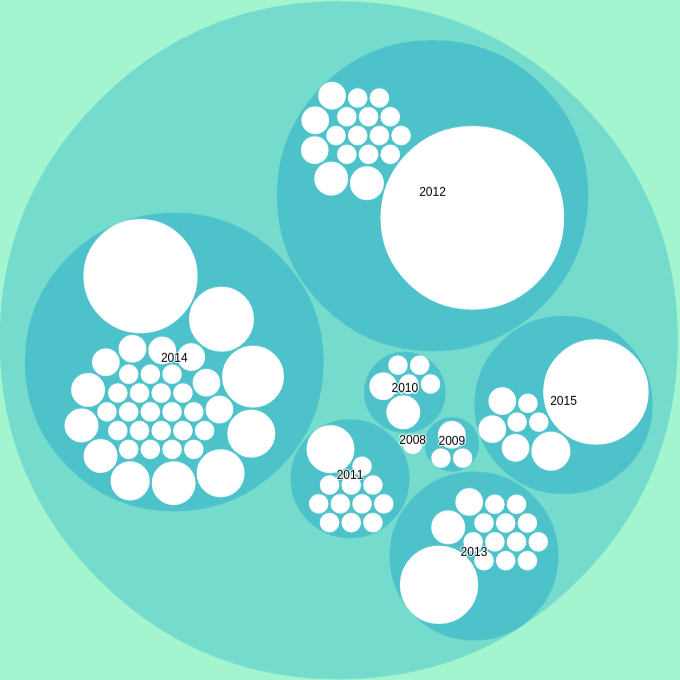
\includegraphics[scale=0.6]{./imagens/zoomable_circle_packing_genre_year_livecoding.png}
\caption{Empacotamento de informações a respeito de gênero musical a partir de anos de produção}
\label{fig:pacotao}
\end{center}
\end{figure}

Os seguintes os termos delimitados foram: \begin{inparaenum}[\itshape a)\upshape]
\item \emph{livecoding}/\emph{live-coding}: dados coerentes com a bibliografia pesquisada\footnote{A exclusão do termo \emph{live code/live coding} foi feita pois a separação criava uma ambiguidade de busca no \emph{Soundcloud}, isto é, \emph{live} poderia não se referir ao que pesquisamos por \emph{livecoding}.};
\item \emph{algorave}/\emph{algopop}: parte considerável da produção do \emph{livecoding} realizada em ambientes noturnos, informais ou de entretenimento (possue relação com o elemento dança);
\item \emph{bytebeat}: parte considerável de uma técnica de programação musical descrita pela primeira vez por \citeonline{heikkila_discovering_2011} e aplicada no \emph{livecoding}, isto é, apenas um fragmento dessa prodção pode se encaixar como \emph{livecoding} (um desses programas é o \emph{Wavepot});
\item \emph{algorithmic music}:música algorítmica, seguindo a subdivisão Música Gerada por Computador, ou \emph{Computer Generated Music}\cite{cope_prefacio_2008}.
\end{inparaenum}

\begin{figure}[h]
\begin{center}
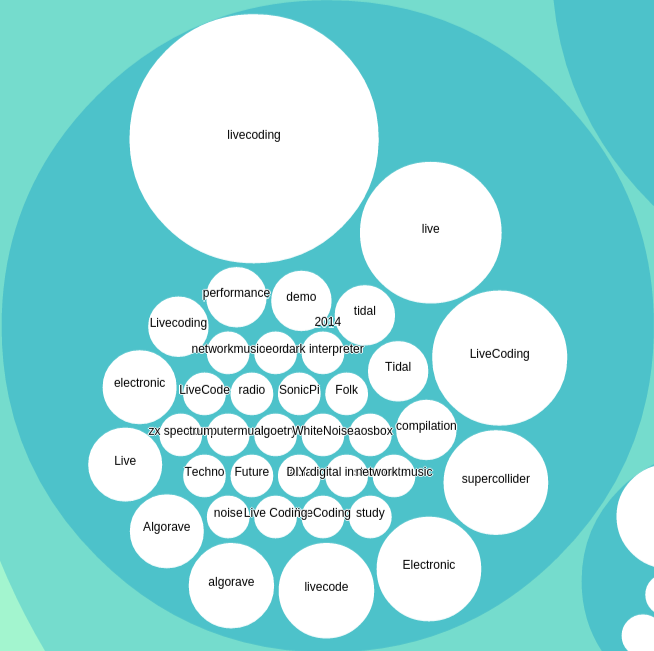
\includegraphics[scale=0.6]{./imagens/zoomable_circle_packing_genre_year_livecoding2.png}
\caption{Detalhamento de informações a respeito de gênero musical a partir de anos de produção}
\label{pacotao2}
\end{center}
\end{figure}

Os dados levantados são de janeiro e fevereiro de 2015; não realizamos mais levantamentos. Os motivos foram: \begin{inparaenum}[\itshape i)\upshape]
\item a dificuldade de análise das assimetrias observadas, que requerem maior experiência com técnicas estatísticas.
\item os dados ilustram as variedades de categorizações musicais no \emph{live coding}. Pode ser interessante observar se tais variedades se aplicam em um único \emph{live coder}.
\end{inparaenum}

\begin{figure}
\begin{center}
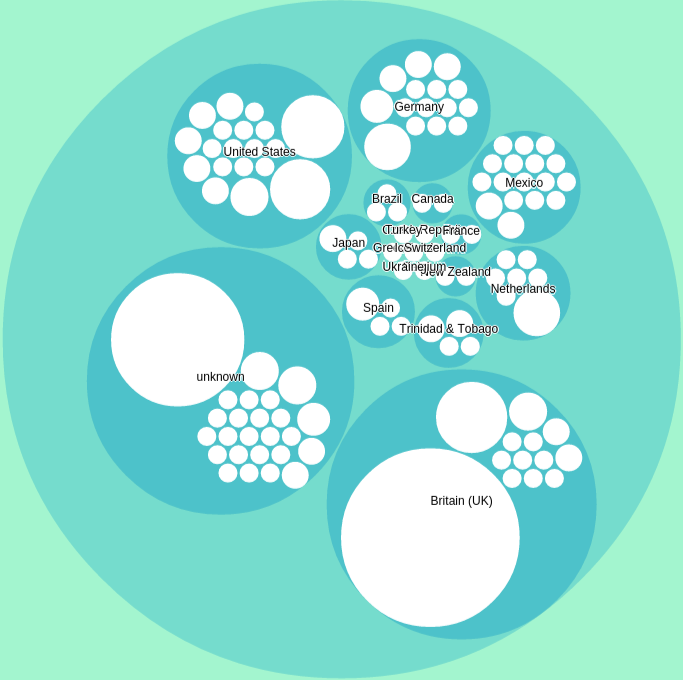
\includegraphics[scale=0.6]{./imagens/zoomable_circle_packing_genre_year_livecoding3.png}
\caption{Empacotamento de informações a respeito de gênero musical a partir de países onde ocorreram as produções}
\label{pacotao3}
\end{center}
\end{figure}

Antes de discutir três casos específicos de um \emph{live coder} (Sorensen), contextualizamos os \emph{live coding} no \autoref{cap:trabalhos_relacionados}. Alguns precedentes históricos do \emph{live coding}, como \emph{GROOVE}, o compositor \emph{Pietro Grossi}, a \emph{Live Computer Music} da Baía de São Franscisco entre os anos 70 e 80 nos Estados Unidos, e a emancipação de uma organização, TOPLAP\footnote{Disponível em \url{http://www.toplap.org}.}, e o destaque de \emph{live coders} ingleses, foram fatores para descrever, neste trabalho, o \emph{live coding} como técnica de improvisação artística original de um Norte político e econômico; delimitar o \emph{live coding} como um Programa de Investigação Científica em universidades; ou descrever o \emph{live coding} como dispositivo de improvisação para replicação de categorizações musicais.

\begin{figure}
\begin{center}
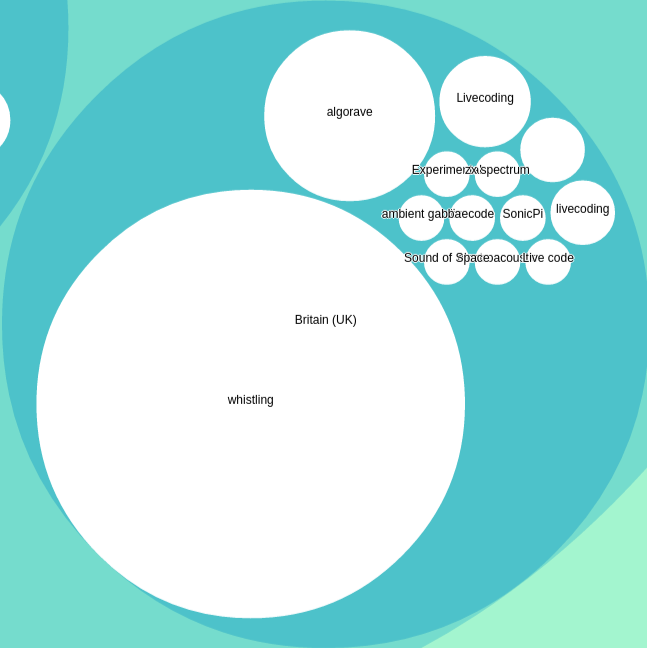
\includegraphics[scale=0.6]{./imagens/zoomable_circle_packing_genre_year_livecoding4.png}
\caption{Detalhamento de informações a respeito de gênero musical a partir de países onde ocorreram as produções.}
\label{pacotao4}
\end{center}
\end{figure}

\section{Justificativa}

A investigação dos precedentes históricos permitem observar o \emph{núcleo de pesquisa} e a \emph{heurística} \cite{lakatos_falsification_1970,neto_lakatos_2008} do \emph{live coding}, e separá-lo, por exemplo, da \emph{live Computer Music}. 

Um paradigma comum entre todos exemplos citados no último parágrafo da seção anterior, dos mais antigos, até os mais atuais, é a utilização de um ou mais computador(es), ou partes deles (microchips),  em um contexto de performance artística. 

Dos exemplos mais atuais, as publicações de manifestos no início dos anos 2000, são considerados, neste trabalho, como os primeiros pontos delimitadores. Tais manifestos incluem, além da Música de processos (de um Steve Reich, Alvin Lucier, ou até mesmo o minimalismo de Philip Glass), O que diferencia este manifesto de seus pr

Para lidar com as liminaridades do \emph{live coding}, as seguintes improvisações foram escolhidas: \begin{inparaenum}[\itshape i)\upshape]
\item \emph{Study in Keith} (2009)\footnote{Disponível em \url{https://vimeo.com/2433947}.}, uma improvisação de códigos que busca replicar o estilo de Keith Jarret);
\item \emph{The Disklavier Sessions} (2010)\footnote{\url{https://vimeo.com/50061269}.}, um \emph{teaser} demostrativo. Demonstra o controle de um piano híbrido da Yamaha, \emph{Disklavier}, para replicar \emph{Jazz} e um \emph{Minimalismo} semelhante a um Steve Reich; 
\item \emph{The Day of Triffords} (2009)\footnote{\url{https://vimeo.com/2735394}.}, ilustração do gênero musical \emph{algorave}, como replicação músicas eletrônicas de ambientes urbanos noturnos.
\end{inparaenum}.

